%%%%%%%%%%%%%%%%%%%%%%%%%%%%%%%%%%%%%%%%%
% Medium Length Graduate Curriculum Vitae
% LaTeX Template
% Version 1.1 (9/12/12)
%
% This template has been downloaded from:
% http://www.LaTeXTemplates.com
%
% Original author:
% Rensselaer Polytechnic Institute (http://www.rpi.edu/dept/arc/training/latex/resumes/)
%
% Important note:
% This template requires the res.cls file to be in the same directory as the
% .tex file. The res.cls file provides the resume style used for structuring the
% document.
%
%%%%%%%%%%%%%%%%%%%%%%%%%%%%%%%%%%%%%%%%%

%----------------------------------------------------------------------------------------
%	PACKAGES AND OTHER DOCUMENT CONFIGURATIONS
%----------------------------------------------------------------------------------------

\documentclass[margin, 10pt]{res} % Use the res.cls style, the font size can be changed to 11pt or 12pt here

\usepackage{helvet} % Default font is the helvetica postscript font
%\usepackage{newcent} % To change the default font to the new century schoolbook postscript font uncomment this line and comment the one above

\setlength{\textwidth}{5.1in} % Text width of the document
\usepackage[utf8]{inputenc}
\usepackage[T1]{fontenc}
\usepackage[final]{pdfpages}
\usepackage[german]{babel}
\begin{document}

%----------------------------------------------------------------------------------------
%	German CV
%----------------------------------------------------------------------------------------
%----------------------------------------------------------------------------------------
%	NAME AND ADDRESS SECTION
%----------------------------------------------------------------------------------------

\moveleft.5\hoffset\centerline{\large\bf Xuan Song} % Your name at the top
\moveleft\hoffset\vbox{\hrule width\resumewidth height 1pt}\smallskip % Horizontal line after name; adjust line thickness by changing the '1pt'
 	
\moveleft.5\hoffset\centerline{Gaertnerweg 28} % Your address
\moveleft.5\hoffset\centerline{Frankfurt am Main 60322 }
\moveleft.5\hoffset\centerline{+49 15770239958}
\moveleft.5\hoffset\centerline{songxuan319@gmail.com}
\moveleft.5\hoffset\centerline{Github: https://github.com/sxuaner}

%----------------------------------------------------------------------------------------
\begin{resume}

%----------------------------------------------------------------------------------------
%	OBJECTIVE SECTION
%----------------------------------------------------------------------------------------
 
\section{Das Ziel}  

%To obtain a chance to begin job career as a programmer with outstanding English and German language skills and target oriented mindset. I am ready to start working immediately.

Mit Verhandlungssicherer Englisch und B2 Stufe Deutsch Sprachekenntnissen möchte ich gern die Karriere als Programmer beginnen. Ich bin 	zielorientiert und kann sofort anfangen zu arbeiten.

%----------------------------------------------------------------------------------------
%	Technology SKILLS SECTION
%----------------------------------------------------------------------------------------

\section{Technologie \\ Fähigkeiten} 

{\sl Programmiersprachen:} 		Java, Groovy \\
{\sl Client-side Technologien:} 	Javascript, PHP\\
{\sl Server-side Technologien:} 	MySQL, Linux OS, Apache Tomcat Web Server, Java Servlet, Jenkins\\
{\sl Andere Technologien:}  		JUnit Test Framework, Git, Latex

%----------------------------------------------------------------------------------------
%	Language Skills
%----------------------------------------------------------------------------------------

\section{Sprachkentnisse} 
{\sl Chinese:} 		Mutter Sprache\\
{\sl English:} 		C1, sehr gut gesprochene Sprache\\
{\sl German:} 		B2, sich verständlich machen können.
%----------------------------------------------------------------------------------------
%	Education SECTION
%----------------------------------------------------------------------------------------
\section{Ausbildung}
{\sl Master Computer Science} \hfill  September.2013 - September.2017\\
High Integrity Systems \\ University of Applied Sciences, Frankfurt am Main(FH FFM)\\
Notenspiegel beigefügt.\\
Masterarbeit: \textit{A data collection system based on quadcopter control and wireless networks}

{\sl Bachelor Computer Science} \hfill September 2009 - June 2013 \\
Henan Normal University, PR China\\
Notenspiegel beigefügt\\
Bachelorarbeit: \textit{A personal blog implemented with Linux, Apache Http server, Mysql database and Wordpress}

%----------------------------------------------------------------------------------------
%	Language Skills
%----------------------------------------------------------------------------------------

\section{Prof. \& andere Arbeitserfahrungen} 
%Kappa Sigma Fraternity, {\sl President} \hfill August 2014 - May 2015\\

%Kappa Sigma Fraternity, {\sl Treasurer} \hfill December 2013 - August 2014 \\
Ende January - Anfang February 2015, 2016, 2017, 2018\\
Englisch \& Deutsch Dolmetscher bei Frankfurt Messe.\\
Thema: \textit{Die Papier Welt} 

Juni.2015 - October 2015\\
Wissenschaftlicher Mitarbeiter bei Netzwerksicherheit Gruppe an der FH FFM 

September.2012 - Januar 2013\\
Pfleger \& Kundendienst bei Xinxiang Jiuzhou Computer Co., Ltd.

%----------------------------------------------------------------------------------------
%	Language Skills
%----------------------------------------------------------------------------------------

\section{Hobbys} 
%Kappa Sigma Fraternity, {\sl President} \hfill August 2014 - May 2015\\
%Kappa Sigma Fraternity, {\sl Treasurer} \hfill December 2013 - August 2014 \\
%Technology Student Association, {\sl Team Leader} \hfill August 2011 - May 2012 \\
Fitness\\
Schwimmen\\
Basketball spielen\\
\clearpage
%----------------------------------------------------------------------------------------
% \includepdf[pages={-},offset=-33mm 0mm]{grades.pdf}
\end{resume}



%----------------------------------------------------------------------------------------
%	NAME AND ADDRESS SECTION
%----------------------------------------------------------------------------------------

\moveleft.5\hoffset\centerline{\large\bf Xuan Song} % Your name at the top
\moveleft\hoffset\vbox{\hrule width\resumewidth height 1pt}\smallskip % Horizontal line after name; adjust line thickness by changing the '1pt'
 	
\moveleft.5\hoffset\centerline{Gaertnerweg 28} % Your address
\moveleft.5\hoffset\centerline{Frankfurt am Main 60322 }
\moveleft.5\hoffset\centerline{+49 15770239958}
\moveleft.5\hoffset\centerline{songxuan319@gmail.com}
\moveleft.5\hoffset\centerline{Github: https://github.com/sxuaner}



%----------------------------------------------------------------------------------------
%	English CV
%----------------------------------------------------------------------------------------

\begin{resume}

%----------------------------------------------------------------------------------------
%	OBJECTIVE SECTION
%----------------------------------------------------------------------------------------
 
\section{OBJECTIVE}  

To begin a career as a programmer with outstanding English, German language skills and goal-oriented mindset. I am ready to start working immediately.
%----------------------------------------------------------------------------------------
%	Technology SKILLS SECTION
%----------------------------------------------------------------------------------------

\section{TECHNOLOGY \\ SKILLS} 

{\sl Programming Languages:} 		Java, Groovy \\
{\sl Client-side Technologies:} 	Javascript, PHP\\
{\sl Server-side Technologies:} 	MySQL, Linux OS, Apache Tomcat Web Server, Java Servlet, Jenkins\\
{\sl Other Technologies:}  		JUnit Test Framework, Git, Latex

%----------------------------------------------------------------------------------------
%	Language Skills
%----------------------------------------------------------------------------------------

\section{LANGUAGE \\ SKILLS} 
{\sl Chinese:} 		Mother Tongue \\
{\sl English:} 		C1, very good spoken language\\
{\sl German:} 		B2
%----------------------------------------------------------------------------------------
%	Education SECTION
%----------------------------------------------------------------------------------------

\section{EDUCATION}

{\sl Master Computer Science} \hfill  September.2013 - September.2017\\
High Integrity Systems \\ University of Applied Sciences, Frankfurt am Main(FH FFM)\\
Grades enclosed.\\
Master Dissertation: \textit{A data collection system based on quadcopter control and wireless networks}

{\sl Bachelor Computer Science} \hfill September 2009 - June 2013 \\
Henan Normal University, PR China\\
Grades enclosed\\
Bachelor Dissertation: \textit{A personal blog implemented with Linux, Apache Http server, Mysql database and Wordpress}

%----------------------------------------------------------------------------------------
%	Language Skills
%----------------------------------------------------------------------------------------

\section{PROFESSIONAL \& OTHER WORKING EXPERIENCE} 
%Kappa Sigma Fraternity, {\sl President} \hfill August 2014 - May 2015\\

%Kappa Sigma Fraternity, {\sl Treasurer} \hfill December 2013 - August 2014 \\
End of January - Beginning of February 2015, 2016, 2017, 2018\\
English \& German Interpreter at The International Fair Frankfurt.\\
Topic "Paper World". 

June.2015 - October 2015\\
Scientific Researcher in Network Security Group at FH FFM 

September.2012 - January 2013\\
Maintenance \& After Sales Service at Xinxiang Jiuzhou Computer Co., Ltd.

%----------------------------------------------------------------------------------------
%	Language Skills
%----------------------------------------------------------------------------------------

\section{HOBBIES \& \\ LEISURE ACTIVITIES} 
%Kappa Sigma Fraternity, {\sl President} \hfill August 2014 - May 2015\\
%Kappa Sigma Fraternity, {\sl Treasurer} \hfill December 2013 - August 2014 \\
%Technology Student Association, {\sl Team Leader} \hfill August 2011 - May 2012 \\
Fitness\\
Swimming\\
Playing Basketball\\

%----------------------------------------------------------------------------------------
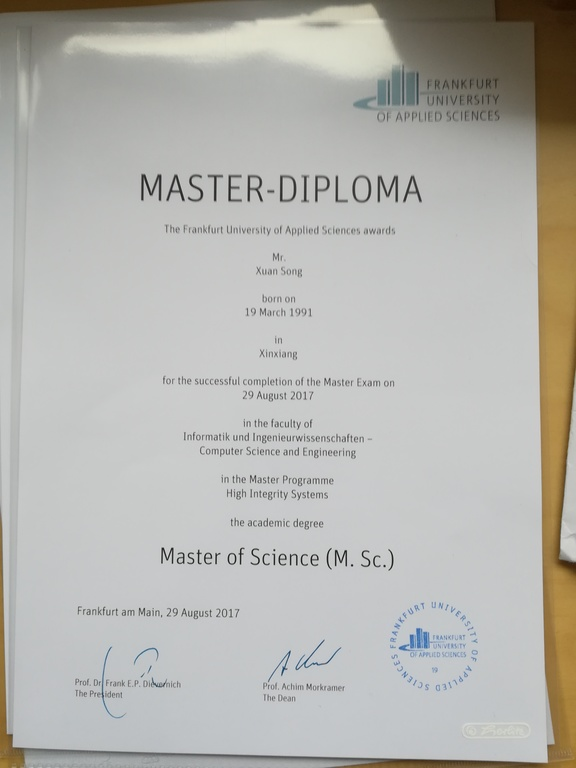
\includepdf[pages={-},offset=-33mm 0mm]{documents/m1.jpg}
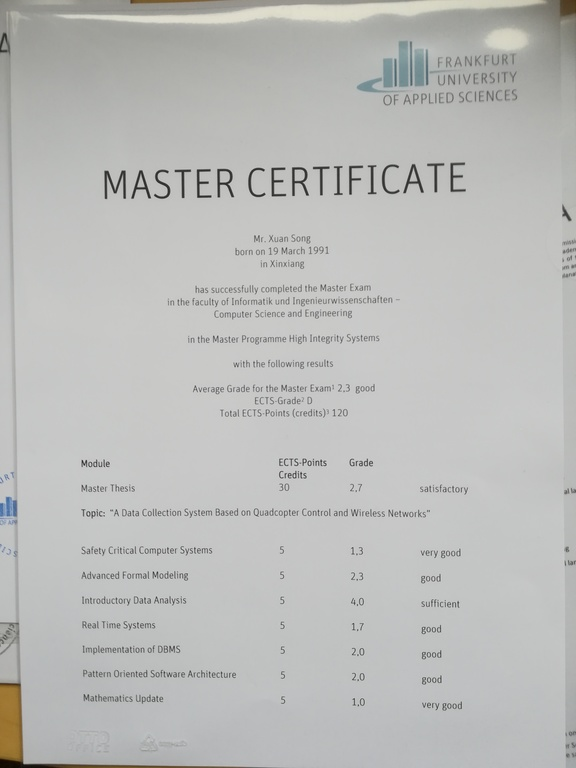
\includepdf[pages={-},offset=-33mm 0mm]{documents/m2.jpg}
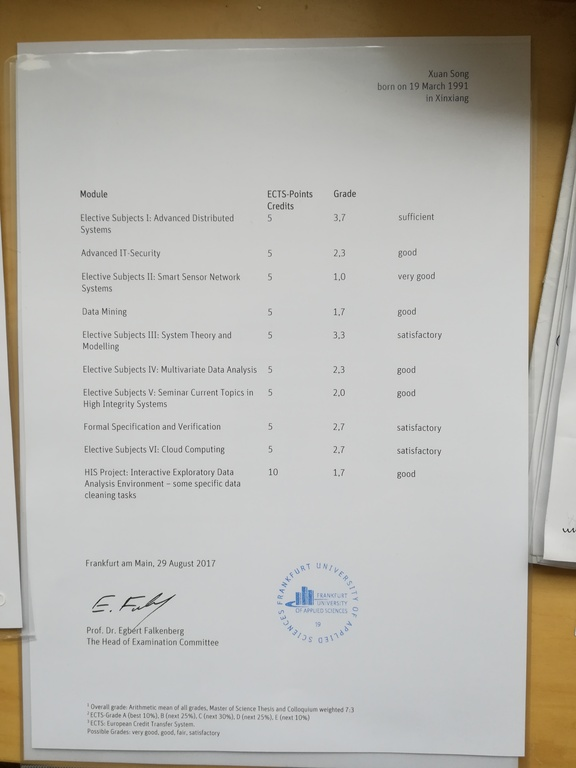
\includepdf[pages={-},offset=-33mm 0mm]{documents/m3.jpg}
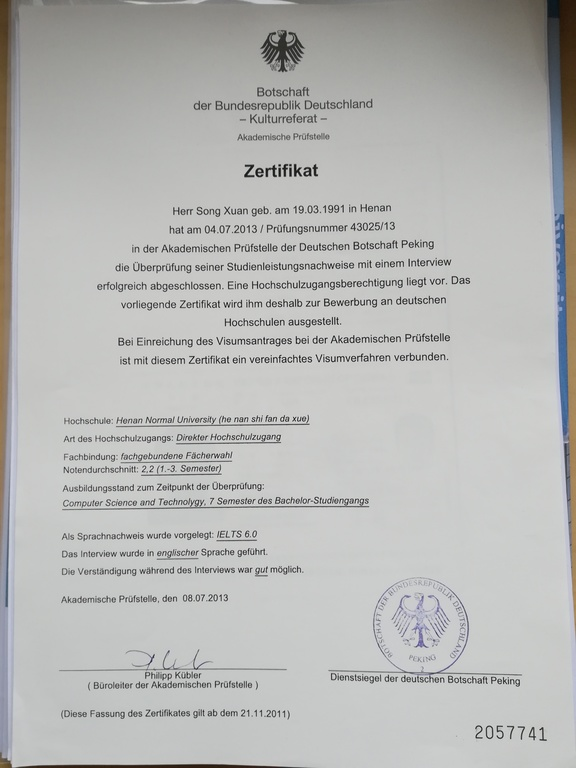
\includepdf[pages={-},offset=-33mm 0mm]{documents/aps.jpg}
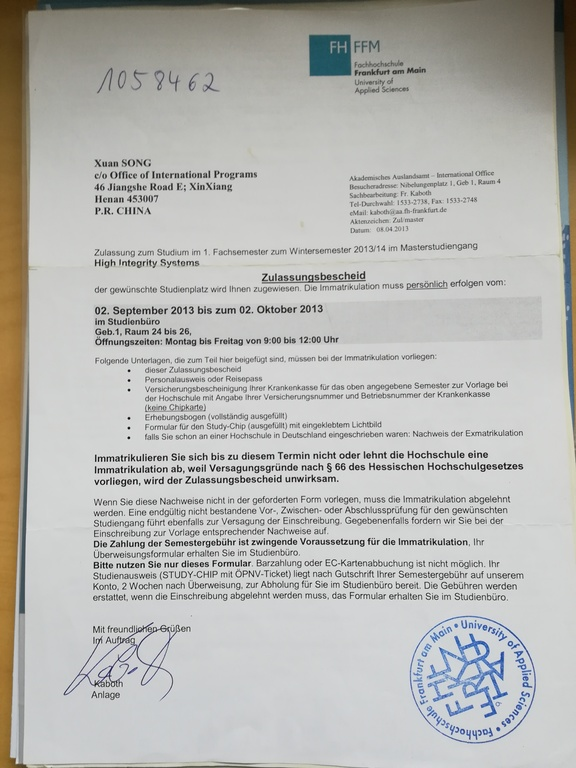
\includepdf[pages={-},offset=-33mm 0mm]{documents/zu.jpg}
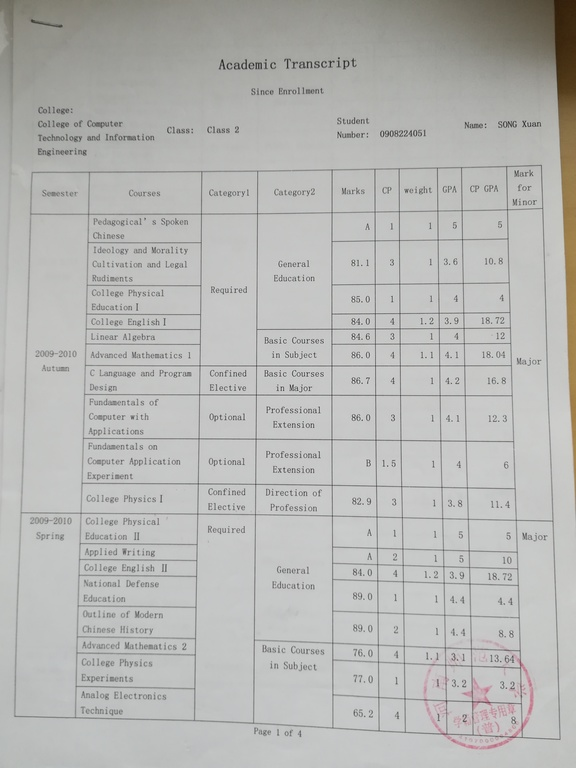
\includepdf[pages={-},offset=-33mm 0mm]{documents/b1.jpg}
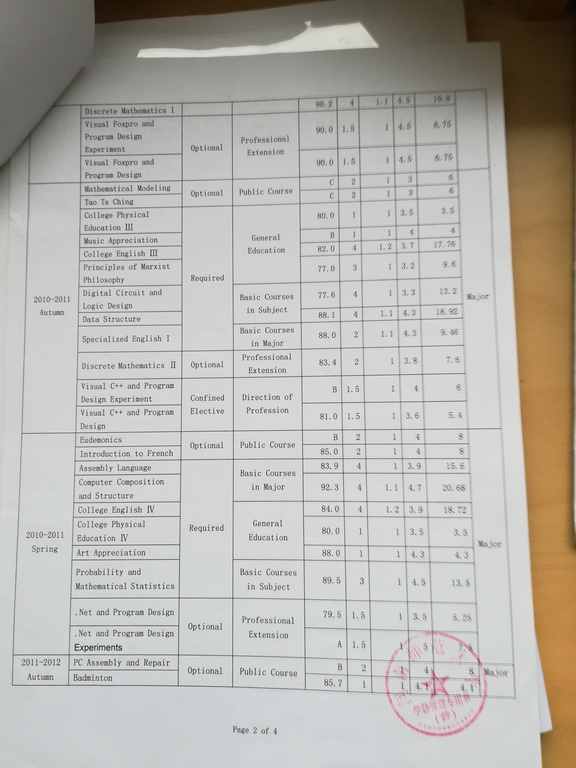
\includepdf[pages={-},offset=-33mm 0mm]{documents/b2.jpg}
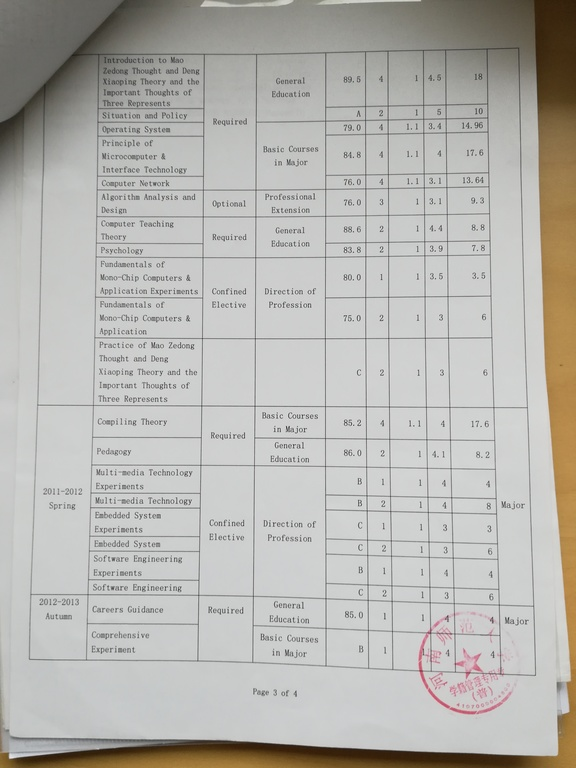
\includepdf[pages={-},offset=-33mm 0mm]{documents/b3.jpg}
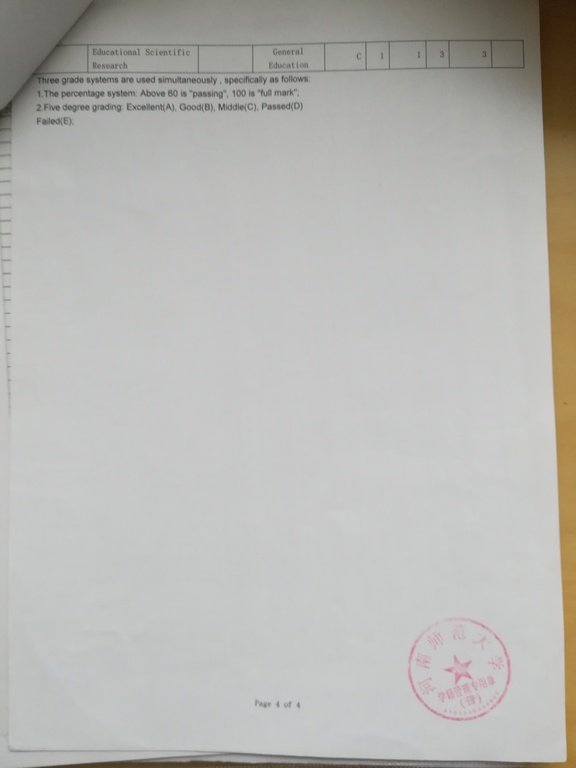
\includepdf[pages={-},offset=-33mm 0mm]{documents/b4.jpg}


\end{resume}
\end{document}